%----------------------------------------------------------------------------------------
%----------------------------------------------------------------------------------------
%----------------------------------------------------------------------------------------
%DATA
%----------------------------------------------------------------------------------------
%----------------------------------------------------------------------------------------
%----------------------------------------------------------------------------------------

\section{DATA}
\label{sec: data}
We used SED templates from K96, to train neural networks.
To test the train networks, we used SED and physical properties of 142 galaxies at 0.5 < $z$ < 1 from T12.
Following of T12 work, we chose these two sets of data to not only show the application of SOMs in SED clustering, but also to easily compare both supervised and unsupervised methods.

 \subsection{Kinney spectral model}
     \begin{figure}
        \centering
        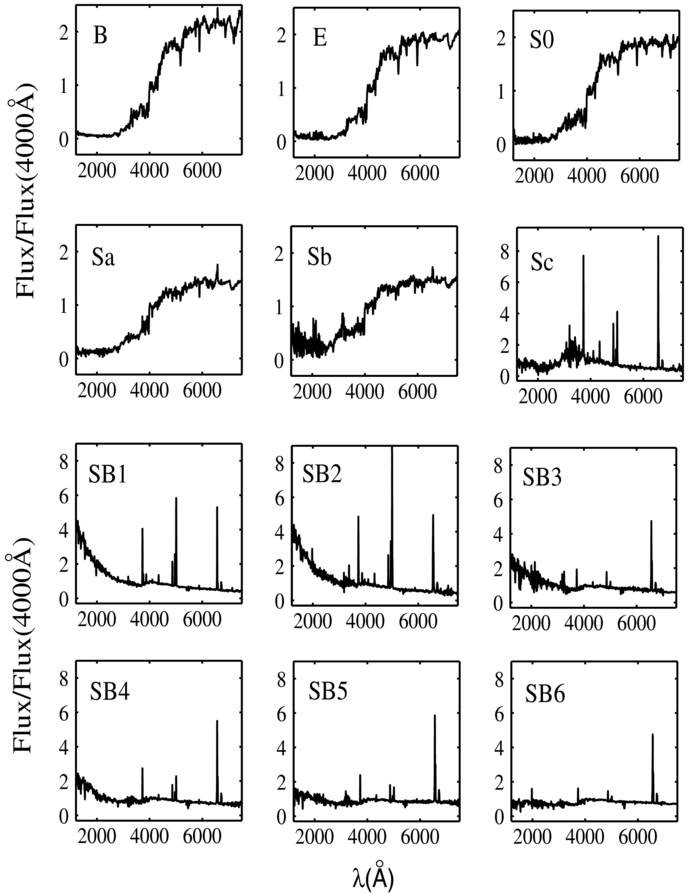
\includegraphics[width=0.5\textwidth]{../images/k96.jpg}
        \caption{K96 spectra template for 12 types of galaxies from T12 paper (Fig. 1 in T12).Type of each template is shown in each frame. Plots B, E, S0, Sa, Sb and SC show spectra that belongs to early type galaxies. Starburst galaxies spectra are indicated with SB 1 to 6. Higher numbers represent more intrinsic colour extinction.}
        \label{fig: k96}
    \end{figure}
     % PB160426: Also, I think you need some stronger arguments for why K96 is a good set of templates to use. Nothing better developed in the last 20 years? 
     %Do they span the whole range of properties you expect the 0.5<z<1.0 galaxies to have?
     %SR: I looked around lots of ppl still using Kinney 96 as a template!
     %20160509PB: You should mention this in a sentence in the next paragraph, something like "These templates are widely used, with a few examples being.."
     %SR: In K96 paper they briefly talked about that you an use these templates to identify the morphological type of galaxies.
      
    K96 used UV-optical spectra of 70 star forming and quiescent nearby galaxies to produce a template that contains 12 types of SEDs.
    This template can be used to classify the SED of the high redshift galaxies. 
    The 12 types of spectra are divided based on their morphological types for early type galaxies or their extinction for starburst galaxies (Fig.~\ref{fig: k96}). 

     % PB160426: I think that's OK, but you will need to look up the journal rules for reproducing a figure from another paper.

    The quiescent group of galaxies includes Bulge (B), Elliptical (E), S0, Sa, Sb, and Sc galaxies.
    Bulge group represents galaxies similar to M31 and M81, which their UV and optical spectroscopy dominated by the stellar population in their bulges.
    
    The starburst galaxies are divided into six groups (SB1 - SB6) based on their intrinsic extinctions ($E(B-V)$). 
    As it is clear in the Fig.~\ref{fig: k96}, SB1 galaxies have lower internal extinctions ($E(B-V) \simeq 0.05$), while SB6 galaxies have the highest amount of extinction ($E(B-V) \simeq 0.65$) among starburst galaxies. %20160509PB: "starburst" is one word
    
    K96 spectra spans from $\sim1200-10000$\AA.
    However, we only used data between $\sim1200-8000$\AA~to train our networks. 
    This wavelength range was chosen due to availability of flux information in those wavelengths for all 12 types of galaxies.
    In early type galaxies' spectra (B to Sb), the spectrum is redder and strong absorption lines, and 4000\AA~break is distinguishable. 
    While SEDs of starburst galaxies are more flat on the optical and NIR part than early type one and show strong emission lines.
    For more details on each spectral type, we encourage readers to see K96 and references therein. 
    

 \subsection{SED and Properties of the sample galaxies} 
    T12 selected 142 galaxies from the spectroscopic campaign of the ESO GOODS-South field, which have a photometry data from the Good-MUSIC catalogue.
    These 142 galaxies were selected due to availability of data from HST/ACS; VLA/ISAAC; and \Spitzer/MIPS and IRAC. 
    Data from these instruments were necessary in order to have a complete picture of stellar population and SFR.
    The photometry data contain data in 10 - 13 filters with the wavelength range of $\sim 0.4-24 \mu$m, in the observed frame. % PB160426: I assume these galaxies have spectroscopic redshifts, or were redshifts derived from photometry? from spectroscopic. 
    They used these photometry data as inputs for Code Investigating GALaxy Emission ({\em CIGALE} code;~\citep[][hereafter N09]{Noll09}) to generate the best fitted SED for each galaxy as well as some of the physical properties of the galaxies.
    
    {\em CIGALE} is a valuable tool to investigate the properties of the galaxy using UV to IR wavebands.
    It uses stellar populations, synthetic attenuation and dust emission models, spectral line templates, and active galactic nuclei's optical spectral templates to model SED of the galaxies.
    This code was successfully tested on data from 39 galaxies selected from the Spitzer Infrared Nearby Galaxy Survey (SINGS;~\citep{Kennicutt03}) by N09.
    T12 produced the best SED match for each galaxy.
    Then, they used an exponentially decreasing SFR, visual attenuation ($\tau$) model and derived physical properties of galaxies such as age, and stellar mass.
    Some of these properties are shown in Tab~\ref{tab: props}.
    They assumed the Salpeter initial mass function~\citep{Salpeter55} and old stellar population age of $\sim 10$~Gyr.
    More details on creating SEDs and extracting information about galaxies properties using {\em CIGALE} can be found in N09 and T12.
    
     For testing the created networks, we used SED produced by T12. 
     However, we only used part of the SEDs that have the same wavelengths as K96 SEDs. %PB160427: need to be more explicit here about exactly what the spectra being analyzed are. Is the data vector for each object a list of fluxes (flux densities) as a function of (rest) wavelength? Same wavelengths for every object? What is the spectral resolution? Do the spectra include the whole galaxy or just the central part?
     %%%%%SR160428: Hossein will write about it.
     In the Sec.~\ref{sec: 1D}, we studied these properties for each categorization.
    
    
    \begin{table}
\caption[]{Description of the properties of T12 galaxies; the output result of {\em CIGALE}}     
\label{tab: props}
\centering
\begin{tabular}{l l l}
\hline\hline
\noalign{\smallskip}
Par. & Unit & Description\\
\noalign{\smallskip}
\hline
\noalign{\smallskip}
$t_{\,\mathrm{oSP}}$ & Gyr & age of old SP model \\
$t_{\,\mathrm{ySP}}$ & Gyr & age of young SP model \\
$f_\mathrm{burst}$ & --- & mass fraction of \\
& & young single population (SP) model \\
\noalign{\smallskip}
$t_{\,\mathrm{D4000}}$ & Gyr & D4000-related age \\
\noalign{\smallskip}
$M_\mathrm{star}$ & M$_\odot$ & total stellar mass  \\
SFR & M$_\odot$/yr & instantaneous SFR  \\
$A_\mathrm{FUV}$ & mag & attenuation at 1500\,\AA{} \\
\noalign{\smallskip}
\hline
\end{tabular}
\end{table}
